Es muy importante considerar la longitud de onda de la onda. Si el tamaño de la abertura es muy superior a la longitud de onda, la onda pasa sin ningún problema. Mientras el tamaño de la abertura se acerca a la longitud de onda la difracción se vuelve más marcada, hasta el punto donde ambos valores son muy parecidos y la curvatura de la onda difractada tiende a ser uniforme. Cuando ambos valores son iguales ocurre una difracción verdadera o completa.

\begin{figure}[H]
  \centering
  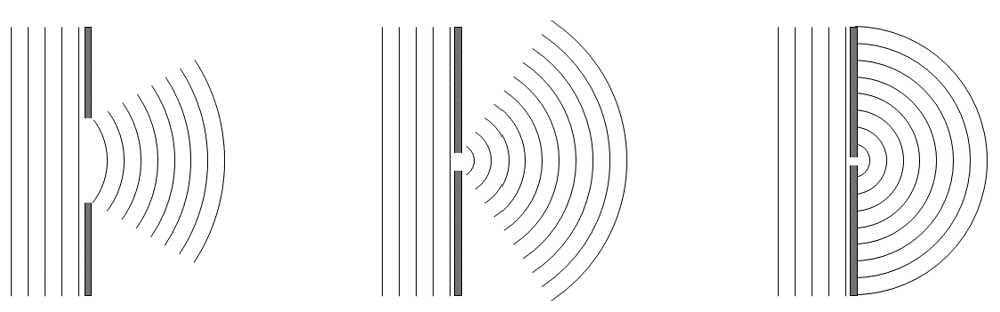
\includegraphics{imagenes/difraccion_atraves.png}
  \caption{Difracción a través de una abertura\cite{xmpdiffraction}}
\end{figure}
